% Paper 1 draft, sections 3-6. Working draft 2026-11-23.
% Numbers trace to: docs/gated_monitor_comparison_results.md, docs/gated_monitor_null_calibration_results.md,
% docs/r7_adaptation_strength_sweep_results.md, scripts/g1_kelly_check.py.

\section{Growth-rate prediction}\label{sec:prediction}

\paragraph{Setting.}
A deployed policy $\pi$ and a reference policy $\pi_{\mathrm{ref}}$ act on a stream of events. The paired
decision cost $c_t = \mathrm{cost}(\pi(X_t),Y_t)-\mathrm{cost}(\pi_{\mathrm{ref}}(X_t),Y_t)\in[-5,5]$ is observed only
when a label is bought. Let $A_t=\mathbf 1[\pi(X_t)\neq\pi_{\mathrm{ref}}(X_t)]$ be the disagreement indicator and $\rho=\Pr(A_t=1)$.
Because the cost depends on the prediction and the label only, $c_t=0$ whenever $A_t=0$. The null is
$\mathbb E[c_t\mid\mathcal F_{t-1}]\le\varepsilon$, and the monitor raises an alarm when a betting e-process crosses $1/\alpha$ for a chosen level $\alpha$.
Labels cost money; the monitor holds a reserve equal to a fraction $r$ of the cost of labelling every event.

\paragraph{Two query rules.}
\emph{Uniform} labelling queries every event with probability $r$, giving the inverse-propensity increment
$Z_t=-\varepsilon+L_tc_t/r$, where $L_t\in\{0,1\}$ records whether the label is bought, with support bound $5/r+\varepsilon$.
The registered uniform comparator (uniform PPI) adds a ridge proxy $h_t$, $Z_t=-\varepsilon+h_t+L_t(c_t-h_t)/r$, with the wider support bound $B_u=5.1(2/r-1)$;
the growth calculation below takes $h_t=0$ under that arm's bound.
\emph{Gated} labelling never queries an agreement, since its cost is known to be zero, and queries a disagreement with
probability $q_t$, giving $Z_t=-\varepsilon+A_tL_tc_t/q_t$ with predictable support bound $B_t=5/q_t+\varepsilon$.
Gating at rate $q_D=\min(1,r\,\bar\kappa_{\mathrm{val}}/\overline{A\kappa}_{\mathrm{val}})$ spends in expectation the same label budget
as uniform labelling at rate $r$, or less when $q_D=1$ ($\kappa_t$ is the price of label $t$, and bars are validation-window means).

\paragraph{Delayed labels.}
Neither gated HT rule uses an outcome to decide what to query or how to bound an increment: the fixed rate comes from validation data, and the paced rate from past disagreements and tariffs.
So if every label arrives $d$ events late and increments are processed in event order, the monitor computes the same e-process $d$ events later.
The guarantee is a statement about that path in event order, so it needs the same condition as before, $\mathbb E[c_t\mid\text{earlier events}]\le\varepsilon$, and query and bound choices that use no outcome; the delay changes only when each term is seen.
Under these, validity is unchanged and each alarm comes exactly $d$ events later; within a fixed window, an alarm due in its last $d$ events falls outside it.

\paragraph{Growth.}
With stake $\lambda$ the e-process multiplies by $1+\lambda Z_t/B_t$, so the per-event growth is
$G(\lambda)=\mathbb E\log(1+\lambda Z_t/B_t)$ and the monitor uses the stake grid $\{0.05,0.1,0.2,0.4,0.8\}$.
For a small signal and an interior optimum, $G\approx\mu^2/(2\,\mathbb E Z^2)$ with $\mu$ the mean excess cost, so the ratio of growth rates is
the ratio of second moments:
\[
\frac{G_{\mathrm{gated}}}{G_{\mathrm{unif}}}\;\approx\;\frac{\mathbb E Z_u^2}{\mathbb E Z_g^2}\;\approx\;
\frac{\rho\,\mathbb E[c^2\mid A{=}1]/r}{\rho\,\mathbb E[c^2\mid A{=}1]/q_D}=\frac{q_D}{r}.
\]
When $q_D=r/\rho<1$ this is $1/\rho$: the gated monitor pays only for events that carry information.
When the budget covers every disagreement ($q_D=1$) it is $1/r$. In both regimes the ratio is
$\min(1/\rho,1/r)$. This is the $1/\rho$ label saving of paired auditing~\citep{discern}, restated as an evidence-growth ratio under a common budget.

\paragraph{Support bounds enlarge the gain.}
A bounded e-process cannot stake more than $B$ allows: with a stake grid capped at $0.8$ the effective bet per unit of $Z$ is $\lambda/B$.
The uniform PPI arm's bound $B_u=5.1(2/r-1)$ is $9$--$24\times$ larger than the gated arm's across the four budgets, so its stakes are
pinned near the cap. Active inverse-propensity e-processes carry the same range condition, $\lambda\le(1/q_{\min}-\theta)^{-1}$, with $\theta$ their risk level~\citep{xu2024active}.
We compute $G$ exactly, enumerating the query coin, for each arm with its own bound and the registered grid on the realised post-onset
paths of the first 20 \texttt{boundary\_local\_harm} comparison streams. Table~\ref{tab:prediction} gives the result.

\begin{table}[t]
\centering\small
\caption{Gated-to-uniform evidence-growth ratio. ``Small-signal'' is $\min(1/\rho,1/r)$ with $\rho=0.084$;
``uncapped'' maximises the stake continuously; ``registered grid'' uses the monitor's stake grid and each arm's support bound.
The registered prediction was made before any monitor run. ``Measured'' and the registered prediction compare against uniform PPI.
``No proxy'' is an exploratory measurement against uniform labelling without a proxy, on CPU streams (Section~\ref{sec:gating}).}
\label{tab:prediction}
\begin{tabular}{lrrrrr@{\qquad}r}
\toprule
$r$ & Small-signal & Uncapped & Reg.\ grid & Reg.\ prediction & Measured & No proxy \\
\midrule
0.02 & 11.9 & 12.4 & 20.0 & 18   & 17.5 & 12.8 \\
0.05 & 11.9 & 12.5 & 19.7 & 18   & 20.6 & 11.5 \\
0.10 & 10.0 & 10.1 & 15.5 & 15   & 14.7 & 9.5 \\
0.20 & 5.0  & 5.1  & 7.6  & 7.5  & 7.2  & 5.1 \\
\bottomrule
\end{tabular}
\end{table}

\begin{figure}[t]
\centering
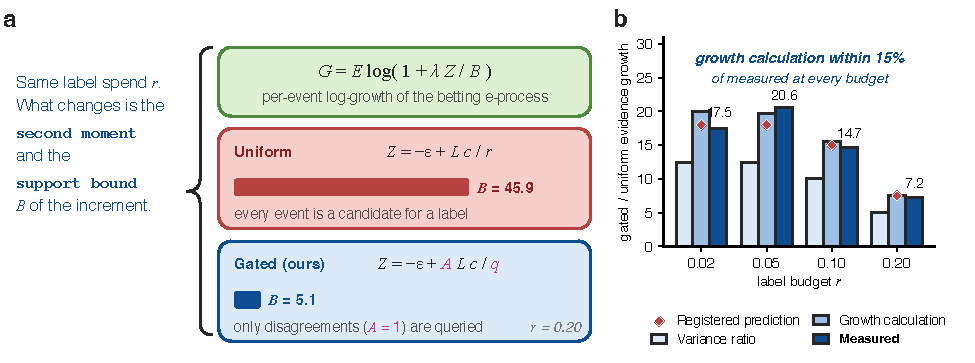
\includegraphics[width=\linewidth]{figures/fig_growth2.pdf}
\caption{The gating gain is predicted within $15\%$ at every label budget. \textbf{a} At the same label budget $r$, gated and uniform labelling differ in the second moment of the increment $Z$ and in its support bound $B$ (bars drawn to scale at $r=0.20$); changed terms are in magenta. The uniform bar is the uniform PPI bound ($45.9$ at $r=0.20$), used with $h_t=0$ as in the growth calculation.
\textbf{b} Gated-to-uniform evidence growth: the variance ratio fixes the order of magnitude, the growth calculation with each arm's bound and the registered stake grid tracks the measured ratio, and the registered prediction (red diamonds) was made before any monitor run.}
\label{fig:growth}
\end{figure}

The variance argument fixes the order of magnitude, and the support bound accounts for the remainder: the registered-grid calculation lands within $15\%$ of the measured ratio at every budget.
Removing the wider bound, the no-proxy column lands near the variance ratio.

\section{Registered protocol}\label{sec:protocol}

\paragraph{Streams.}
Synthetic streams have $n=3200$ events and $d=16$ features. Events $0$--$399$ train the learner, $400$--$799$ are the validation window that seeds pacing and the proxy, and the monitor runs from event $800$.
The deployed classifier uses a fixed $0.5$ threshold; the reference is the cost-minimising rule
(false-negative cost $5$, false-positive cost $1$, tariffs in $[0.5,2.5]$, tolerance $\varepsilon=0.1$, $\alpha=0.05$).
Scenarios are \texttt{stationary} and \texttt{benign\_nuisance} (null controls), \texttt{boundary\_local\_harm}
(an adverse conditional-mean increase localised near the source decision boundary), and \texttt{harmful\_adaptation}
(stationary outcomes, with a policy intervention at event $1600$ that sets actions positive and lifts disagreement from about $9\%$ to $42\%$ on the comparison streams).

\paragraph{Arms.}
Gated: Horvitz--Thompson (HT) at a fixed rate $q_D$ (\texttt{gated\_ht\_fixed}) and at an online-paced rate from a past-only $200$-event tariff window,
clipped to $[0.10,1]$ (\texttt{gated\_ht\_paced}); a proxy-anchored variant; an empirical-Bernstein engine.
Ungated: uniform labelling with a ridge proxy (prediction-powered inference, PPI~\citep{angelopoulos2023ppi}), and the variance-allocated policy.
Published and composed comparators: Timans GRAPA (growth-rate adaptive betting~\citep{waudbysmith2024}), the prediction-powered e-value (PPE)~\citep{csillag2025}, and Xu active betting~\citep{xu2024active},
each given the same gating, correct bounds, label-dollar cap, query coins and proxy access.
A label-free feature-drift sentinel is recorded as a distribution-shift diagnostic; it targets a different null and is not ranked.
Full feedback and a never-alarming monitor are unmatched references.
The reserve is a hard stop: processing ends when the remaining budget falls below the largest label price.

\paragraph{Registration.}
The protocol, the regime map with falsification criteria, the comparator panel and the seed blocks were frozen by hash before the first registered stream.
Calibration used $2{,}000$ streams per null scenario and budget cell with a simultaneous exact $5\%$ bound per arm.
The comparison used $100$ fresh streams per scenario and budget (seeds $58400000$--$58400099$) with two co-primary endpoints:
the post-onset growth ratio at $r=0.20$ (one-sided $97.5\%$ lower bound $\ge2$) and the paired detection difference at $r=0.05$ (lower bound $>0$).
A fidelity stage reproduced the historic uniform-PPI crossings (6/60 at bound 96.9, 47/60 at bound 45.9) exactly before any fresh stream was generated.
One numerical-tolerance amendment was recorded before any comparison outcome was available: an increment that exceeds its support bound
by floating-point rounding (at most $10^{-9}$ relative) is set to the bound. The estimand, arms, thresholds and seeds are unchanged.

\section{Gating results}\label{sec:gating}

\paragraph{Validity.}
In the null cells, the paced gated-HT arm raised between $0$ and $6$ alarms per $2{,}000$ streams, with a largest simultaneous exact upper bound of $0.764\%$.
Every registered arm passed the $5\%$ bound; the largest upper bound anywhere was $1.953\%$ (the PPE source-factor alias, $24/2{,}000$).

\paragraph{Co-primary endpoints.}
Both pass. At $r=0.20$ the paced gated monitor's growth is $7.20\times$ the correctly bounded uniform PPI monitor's (95\% interval $6.88$--$7.55$).
At $r=0.05$ gating wins $100$ discordant streams and loses none (McNemar one-sided $p=7.9\times10^{-31}$).
Table~\ref{tab:r05} lists detection, delay and labels at about equal spend.
At $r=0.20$ the budget exceeds the disagreement rate, so gating labels every disagreement and leaves budget unused: in the CPU replication it uses $207$ labels against uniform labelling's $471$.

\begin{table}[!h]
\centering
\caption{\texttt{boundary\_local\_harm}, $r=0.05$, 100 streams.}
\label{tab:r05}
\begin{tabular}{lrrr}
\toprule
Arm & Detection & Censored delay & Labels \\
\midrule
gated HT, paced & 1.00 & 496 & 118 \\
gated HT, paced + Timans GRAPA & 1.00 & 469 & 118 \\
PPE gated & 0.99 & 451 & 118 \\
uniform PPI (bound 45.9) & 0.00 & 1{,}616 & 114 \\
uniform PPI + Timans GRAPA & 0.01 & 1{,}611 & 114 \\
Xu active & 0.00 & 1{,}616 & 115 \\
\bottomrule
\end{tabular}
\end{table}

\paragraph{Replication.}
We reran the comparison's seeds on a second random generator (CPU in place of CUDA), which gives new streams. Both co-primary endpoints pass again:
the growth ratio at $r=0.20$ is $7.77\times$ ($95\%$ interval $7.38$--$8.20$) and gating wins $100$ discordant streams to none at $r=0.05$.
The measured ratios across budgets ($21.4/19.1/15.2/7.8$) are within $7\%$ of the growth calculation of Table~\ref{tab:prediction} and within $19\%$ of the registered prediction.
At $r\le0.05$ gated HT arms detect $0.80$ to $1.00$ and the registered ungated arms at most $0.03$.
Null calibration also passes again on $2{,}000$ streams per cell: the paced gated-HT arm raises $1$ to $5$ alarms (largest simultaneous exact upper bound $0.689\%$), and every arm stays below the $5\%$ bound (largest $2.139\%$).

\paragraph{Uniform labelling without a proxy.}
In an exploratory follow-up on the same CPU streams, we added uniform HT labelling without a proxy, under its own bound $5/r+\varepsilon$ and with the same queries and labels as uniform PPI.
The gated-to-uniform growth ratio is then $12.8/11.5/9.5/5.1$ across the four budgets, within $8\%$ of the small-signal value $\min(1/\rho,1/r)$ (Table~\ref{tab:prediction}):
this is the gain from gating itself. The proxy arm's growth is a further $1.5$ to $1.7$ times lower, which accounts for the larger ratio against it.
On \texttt{boundary\_local\_harm} at $r=0.05$, gated HT detects $1.00$ and uniform HT $0.06$ ($0.16$ with Timans GRAPA), with no stream on which uniform HT alone detects.
Under \texttt{harmful\_adaptation}, where the post-intervention disagreement rate of about $0.41$ puts $\min(1/\rho,1/r)$ near $2.4$,
gated HT leads at $r=0.10$ ($0.80$ against $0.46$; $0.87$ against $0.53$ with GRAPA);
at $r=0.05$ it leads with the registered engine ($0.20$ against $0.05$) and is indistinguishable with GRAPA ($0.23$ against $0.28$; two-sided McNemar $p=0.44$).
Uniform HT raised no alarm in the null cells ($100$ streams each).

\paragraph{The prediction at other disagreement rates.}
In a further exploratory study we changed the disagreement rate through the deployed threshold ($0.35$ in place of $0.5$) and through the intervention strength ($s=0.50,0.75,1$), in two blocks of $2{,}400$ fresh streams each (seeds $63100000$--$63100099$ and $63200000$--$63200099$ per setting).
Before each block we fixed the prediction $q/r$ against uniform HT without a proxy, with $q=\min\{1,\max(0.10,r/\rho)\}$, which equals $\min(1/\rho,1/r)$ unless the pacer's floor binds, and a $15\%$ tolerance.
Here $\rho$ is the post-onset disagreement rate; it needs no labels, though under an intervention it is seen only once the intervention happens.
Measured growth takes the best fixed stake per stream on the common post-onset window, averaged over streams.
Before the second block we added a second estimator with less room for hindsight: one stake per arm per cell, chosen on the average over the $100$ streams.
All ten cells at $r\ge0.10$ are within tolerance with the per-stream estimator in both blocks, and with the one-stake estimator in the second (Table~\ref{tab:rho}).
Over all $20$ cells, the per-stream estimator is within tolerance in $15$ in each block and the one-stake estimator in $17$ of the second;
of its three remaining cells, two are above the prediction (by $16\%$ and $18\%$) and one, where the floor binds, is $22\%$ below.
Intervals (Table~\ref{tab:rhoci}) are widest at the smallest budgets (setting A at $r=0.02$: $13$--$60$ for the one-stake estimate).
Gated detection is at least uniform detection in every cell of both blocks, and no arm alarmed in the stationary check at threshold $0.35$.

\begin{table}[!h]
\centering\small
\caption{The gain tracks its prediction at budgets of $10\%$ or more across disagreement rates. Entries are gated-to-uniform (no proxy) growth ratios; $\rho$ and ``predicted'' are from the second block (first-block predictions are within $3\%$ of them); each block is judged against its own prediction. ``One stake'' picks one grid stake per arm per cell. $\dagger$ outside the $15\%$ tolerance; $*$ pacer floor binds.}
\label{tab:rho}
\begin{tabular}{llcccc}
\toprule
Setting & Row & $r=0.02$ & $r=0.05$ & $r=0.10$ & $r=0.20$ \\
\midrule
A: threshold $0.35$, $\rho=0.05$ & predicted & 19.6 & 19.6 & 10.0 & 5.0 \\
 & first block & $10.4^\dagger$ & $14.8^\dagger$ & 9.8 & 5.0 \\
 & second block & $12.5^\dagger$ & $15.8^\dagger$ & 8.6 & 5.0 \\
 & second, one stake & $22.6^\dagger$ & 22.4 & 9.8 & 5.3 \\
\addlinespace
B: registered pair, $\rho=0.09$ & predicted & 11.6 & 11.6 & 10.0 & 5.0 \\
 & first block & $9.1^\dagger$ & 12.3 & 10.0 & 5.1 \\
 & second block & 10.6 & $13.4^\dagger$ & 9.8 & 5.1 \\
 & second, one stake & 11.3 & $13.7^\dagger$ & 9.8 & 5.1 \\
\addlinespace
C: $s=0.50$, $\rho=0.25$ & predicted & 5.0$^*$ & 4.0 & 4.0 & 4.0 \\
 & first block & $3.5^\dagger$ & $3.3^\dagger$ & 3.8 & 3.9 \\
 & second block & $3.4^\dagger$ & 3.9 & 3.8 & 3.6 \\
 & second, one stake & $3.9^\dagger$ & 4.1 & 3.8 & 3.7 \\
\addlinespace
D: $s=0.75$, $\rho=0.33$ & predicted & 5.0$^*$ & 3.0 & 3.0 & 3.0 \\
 & first block & 4.4 & 3.1 & 3.1 & 3.1 \\
 & second block & $4.0^\dagger$ & 3.1 & 3.2 & 3.1 \\
 & second, one stake & 4.6 & 3.2 & 3.2 & 3.2 \\
\addlinespace
E: $s=1$, $\rho=0.41$ & predicted & 5.0$^*$ & 2.4 & 2.4 & 2.4 \\
 & first block & 4.5 & 2.5 & 2.7 & 2.5 \\
 & second block & 4.8 & 2.7 & 2.7 & 2.7 \\
 & second, one stake & 5.3 & 2.7 & 2.7 & 2.7 \\
\bottomrule
\end{tabular}
\end{table}

\paragraph{Predicting the alarm time.}
The growth quantities also give a time. For each grid stake let $g_0$ and $g_1$ be the expected per-event log-growth before and after onset, at each period's query rate and with the query coin enumerated; the predicted alarm is the first post-onset event $T$ at which
$\tfrac15\sum_\lambda \exp\{800\,g_0(\lambda)+T\,g_1(\lambda)\}\ge 1/\alpha$.
The rule has no fitted parameter. Its inputs come from labelled pilot streams that include the post-change distribution, as in a power analysis.
We computed $T$ from the paths of the first block for $40$ arm-cells (one arm, gated or uniform, in one of five settings at one of four budgets) and, before opening the second block's results, fixed the reading:
$T\le800$ means detection at least $0.8$ and a median censored delay within $25\%$ of $T$; $T>1600$, beyond the window, means detection below $0.5$; in between there is no claim.
The reading holds in $28$ of the $32$ arm-cells that carry a claim ($3$ of $4$ delay claims, $25$ of $28$ non-detection claims; $16$ of $16$ uniform and $12$ of $16$ gated).
All four failures are on the safe side, with gated monitors doing better than predicted near a band edge: predicted times of $1{,}641$ and $1{,}693$ with detection $0.53$--$0.66$, and one alarm $26\%$ earlier than predicted.
Observed afterwards, gated monitors with a median alarm inside the window alarmed $7$--$26\%$ earlier than predicted, so for them the rule errs towards over-provisioning a budget.

\paragraph{Registered regimes.}
The regime map predicted that past-paced gating would hold coverage better than a fixed rate when disagreement rises (regime R7). Under \texttt{harmful\_adaptation} the simpler fixed rate was equal or better in detection at every budget
($0.86$ against $0.76$ at $r=0.10$). Section~\ref{sec:pacing} follows up this result and identifies what each rule is good for.

\paragraph{Panel.}
Every gated arm dominates every registered ungated arm at scarce budgets: at $r\le0.05$ gated arms detect $0.82$--$1.00$ and the registered ungated arms $0.00$--$0.01$.
The strongest selective-label arms are gated HT or PPI with Timans GRAPA and the gated PPE alias (mean detection $0.99$).
When the budget covers all disagreements ($q_D=1$) the regime map predicts, and the results confirm, that every gated variant ties: proxies and allocation rules have nothing left to act on.
The PPI proxy adds nothing over gated HT in \texttt{boundary\_local\_harm} and lowers detection under \texttt{harmful\_adaptation} (mean $0.36$--$0.39$ against $0.50$--$0.59$).

\section{Pacing and the label reserve}\label{sec:pacing}

Under a policy intervention the disagreement rate rises, and the monitor must choose between a fixed gating rate set from validation data and a past-paced rate that lowers $q$ as disagreements arrive.
We vary the intervention strength $s$, the probability that a post-intervention event is forced to the positive action
($s\in\{0.10,0.25,0.50,0.75,1.00\}$; disagreement $0.09$ before onset and $0.12$--$0.41$ after it on these sweep streams), across the four budgets with $100$ fresh streams per cell (seeds $61000000$--$61000099$, $2{,}000$ streams in all).

\begin{figure}[t]
\centering
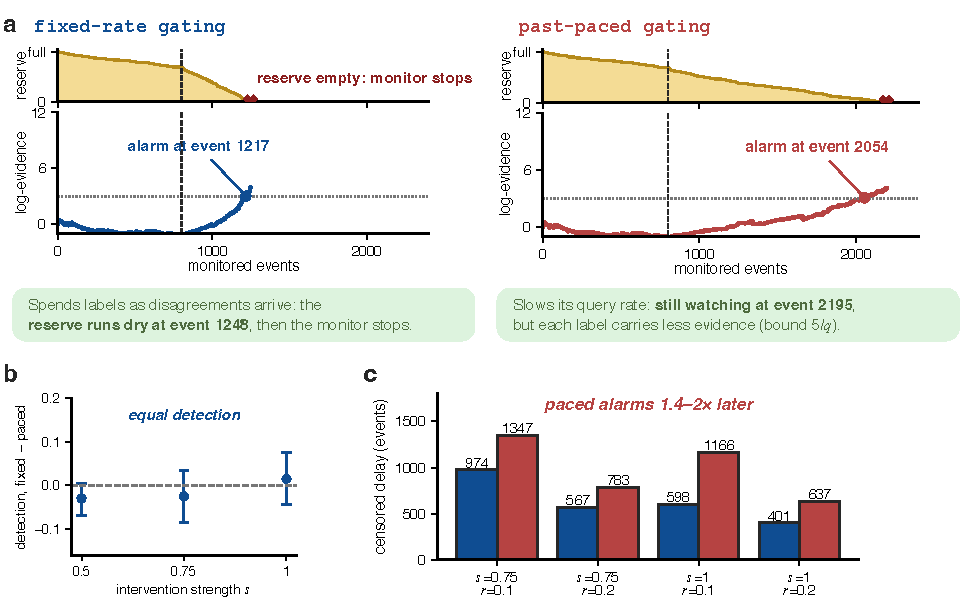
\includegraphics[width=0.86\linewidth]{figures/fig_pacing2.pdf}
\caption{Pacing trades detection delay for monitoring horizon at similar detection rates. \textbf{a} One registered \texttt{harmful\_adaptation} stream ($s=1$, $r=0.10$, seed $61000000$): the fixed-rate monitor's label reserve runs dry at event $1{,}248$ and it alarms at $1{,}217$; the paced monitor is still watching at event $2{,}195$ and alarms at $2{,}054$.
\textbf{b} Pooled over $r\in\{0.05,0.10\}$ and $s\ge0.5$ (100 seeds per cell), fixed minus paced detection has a bootstrap $95\%$ interval containing zero at every strength. \textbf{c} Censored detection delay where both monitors detect.}
\label{fig:pacing}
\end{figure}

\paragraph{Pooled detection is similar with and without pacing.}
Pooled over the $1{,}900$ harm-path rows, fixed minus paced detection is $+0.005$ (bootstrap $95\%$ interval $-0.006$ to $+0.016$) with the registered betting engine
and $-0.006$ ($-0.018$ to $+0.006$) with Timans GRAPA (Table~\ref{tab:pacing}).

\begin{table}[!h]
\centering
\caption{Fixed and paced gating at full intervention strength ($s=1.00$), registered betting engine.
Horizon is events processed before the reserve stops the monitor (of 2{,}400). Censored delay is reported for the two budgets where detection is high.}
\label{tab:pacing}
\begin{tabular}{lrrrrrr}
\toprule
 & \multicolumn{2}{c}{Detection} & \multicolumn{2}{c}{Horizon} & \multicolumn{2}{c}{Censored delay} \\
$r$ & fixed & paced & fixed & paced & fixed & paced \\
\midrule
0.02 & 0.06 & 0.04 & 1{,}131 & 1{,}485 & -- & -- \\
0.05 & 0.19 & 0.22 & 1{,}136 & 2{,}111 & -- & -- \\
0.10 & 0.81 & 0.75 & 1{,}220 & 2{,}274 & 598 & 1{,}166 \\
0.20 & 0.99 & 0.99 & 1{,}793 & 2{,}400 & 401 & 637 \\
\bottomrule
\end{tabular}
\end{table}

\paragraph{Pacing buys horizon.}
The reserve is a hard stop, so a monitor that spends labels faster than its budget accrues stops earlier.
At full strength and $r=0.05$ the fixed monitor processes $1{,}136$ of $2{,}400$ events and the paced monitor $2{,}111$, at $119$ labels each.
Pacing lowers the post-onset query rate from $0.58$ to $0.14$.
The fixed monitor's horizon shrinks monotonically with $s$ at every budget (at $r=0.02$, $1{,}929\to1{,}131$); the paced monitor's shrinks more slowly.

\begin{figure}[t]
\centering
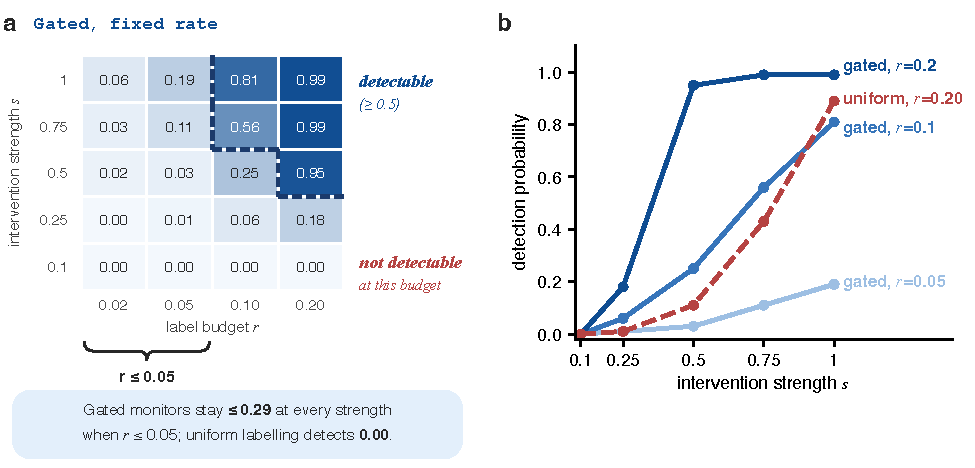
\includegraphics[width=0.86\linewidth]{figures/fig_map2.pdf}
\caption{Gated monitors detect the harm once the budget reaches the disagreements the intervention creates. \textbf{a} Detection probability by label budget and intervention strength under \texttt{harmful\_adaptation} (100 streams per cell); the dashed line encloses cells with detection at least $0.5$, and at $r\le0.05$ no gated variant passes $0.29$ at any strength (the fixed rate shown reaches $0.19$). \textbf{b} Detection against strength for three budgets (gated, blue) and for uniform PPI at $r=0.20$ (red, dashed); uniform PPI detects $0.00$ at $r\le0.05$.}
\label{fig:map}
\end{figure}

\paragraph{Pacing lengthens delay.}
A lower $q$ raises the support bound $5/q$, so each label carries less evidence: the range penalty of Section~\ref{sec:prediction} acting on time.
At full strength, censored delay is $598$ (fixed) against $1{,}166$ (paced) events at $r=0.10$, and $401$ against $637$ at $r=0.20$; at $s=0.75$ it is $974$ against $1{,}347$ and $567$ against $783$.
Fixed gating is the faster detector whenever the budget can afford its disagreements; pacing is the choice only when the monitor must keep running past the burst.

\paragraph{A higher floor tunes the trade-off.}
In an exploratory follow-up, chosen after the sweep and run on $100$ fresh streams per cell (seeds $62000000$--$62000099$; $s\in\{0.75,1\}$), we raised the
pacer's floor on $q$ from $0.10$ to $0.40$. At $r=0.10$ censored delay falls from $1{,}352$ to $1{,}226$ events at $s=0.75$ and from $1{,}194$ to $945$ at $s=1$,
detection stays similar ($0.55$ to $0.56$, and $0.79$ to $0.77$), and the monitor still processes about $1.5\times$ as many events as fixed gating, which remains the faster detector (censored delay $917$ and $769$).
At $r=0.05$ the delay gain is smaller ($3$--$7\%$), and at $r=0.20$ the floor has no material effect. The floor is therefore a dial between delay and horizon
that a deployment can set in advance.

\paragraph{A detectability map.}
Full feedback detects from $s=0.50$ ($0.95$). The primary gated HT arms reach $0.87$--$0.99$ at $r=0.20$ for $s\ge0.50$ (fixed rate $0.95$--$0.99$), and $0.56$--$0.86$ at $r=0.10$ for $s\ge0.75$.
At $r\le0.05$ they reach at most $0.29$ at every strength, where uniform PPI detects $0.00$.
Each cell has $100$ streams, so an exact $95\%$ interval extends at most about $10$ points either side (paced $0.87$: $0.79$--$0.93$).
Detection rises with both the budget and the intervention strength.
Pre-onset alarm rates stay at or below $1/100$ per cell for every primary arm (exact $95\%$ upper bound $4.7\%$); the PPE alias has one cell at $3/100$.
